%  LaTeX support: latex@mdpi.com
%  For support, please attach all files needed for compiling as well as the log file, and specify your operating system, LaTeX version, and LaTeX editor.

%=================================================================
\documentclass[engproc, submit, article,pdftex,moreauthors]{Definitions/mdpi}
% For posting an early version of this manuscript as a preprint, you may use "preprints" as the journal and change "submit" to "accept". The document class line would be, e.g., \documentclass[preprints,article,accept,moreauthors,pdftex]{mdpi}. This is especially recommended for submission to arXiv, where line numbers should be removed before posting. For preprints.org, the editorial staff will make this change immediately prior to posting.
%--------------------
% Class Options:
%--------------------
%---------
% article
%---------
% The default type of manuscript is "article", but can be replaced by:
% abstract, addendum, article, book, bookreview, briefreport, casereport, comment, commentary, communication, conferenceproceedings, correction, conferencereport, entry, expressionofconcern, extendedabstract, datadescriptor, editorial, essay, erratum, hypothesis, interestingimage, obituary, opinion, projectreport, reply, retraction, review, perspective, protocol, shortnote, studyprotocol, systematicreview, supfile, technicalnote, viewpoint, guidelines, registeredreport, tutorial
% supfile = supplementary materials

%----------
% submit
%----------
% The class option "submit" will be changed to "accept" by the Editorial Office when the paper is accepted. This will only make changes to the frontpage (e.g., the logo of the journal will get visible), the headings, and the copyright information. Also, line numbering will be removed. Journal info and pagination for accepted papers will also be assigned by the Editorial Office.

%=================================================================
% MDPI internal commands
\firstpage{1}
\makeatletter
\setcounter{page}{\@firstpage}
\makeatother
\pubvolume{1}
\issuenum{1}
\articlenumber{0}
\pubyear{2025}
\copyrightyear{2025}
%\externaleditor{Academic Editor: Firstname Lastname}
\datereceived{}
%\daterevised{} % Only for the journal Acoustics
\dateaccepted{}
\datepublished{}
%\datecorrected{} % Corrected papers include a "Corrected: XXX" date in the original paper.
%\dateretracted{} % Corrected papers include a "Retracted: XXX" date in the original paper.
\hreflink{https://doi.org/} % If needed use \linebreak
%\doinum{}
%------------------------------------------------------------------
% The following line should be uncommented if the LaTeX file is uploaded to arXiv.org
%\pdfoutput=1

%=================================================================
% Add packages and commands here. The following packages are loaded in our class file: fontenc, inputenc, calc, indentfirst, fancyhdr, graphicx, epstopdf, lastpage, ifthen, lineno, float, amsmath, setspace, enumitem, mathpazo, booktabs, titlesec, etoolbox, tabto, xcolor, soul, multirow, microtype, tikz, totcount, changepage, attrib, upgreek, cleveref, amsthm, hyphenat, natbib, hyperref, footmisc, url, geometry, newfloat, caption

\usepackage{amssymb}
\setcounter{tocdepth}{3}
\usepackage{graphicx}

\usepackage{url}

\usepackage[english]{babel}
%\usepackage[russian]{babel}
\let\vec=\mathbf

\graphicspath{{fig/}}

%----------------------------------------------------------------
\usepackage{bm}
\usepackage{amsfonts}

%\usepackage{subcaption}

\usepackage{tikz}
\usetikzlibrary{decorations.pathreplacing}

%new calligraphic font for subspaces
\usepackage{euscript}
\newcommand{\cA}{\EuScript{A}}
\newcommand{\cB}{\EuScript{B}}
\newcommand{\cC}{\EuScript{C}}
\newcommand{\cD}{\EuScript{D}}
\newcommand{\cE}{\EuScript{E}}
\newcommand{\cF}{\EuScript{F}}
\newcommand{\cG}{\EuScript{G}}
\newcommand{\cH}{\EuScript{H}}
\newcommand{\cI}{\EuScript{I}}
\newcommand{\cJ}{\EuScript{J}}
\newcommand{\cK}{\EuScript{K}}
\newcommand{\cL}{\EuScript{L}}
\newcommand{\cM}{\EuScript{M}}
\newcommand{\cN}{\EuScript{N}}
\newcommand{\cO}{\EuScript{O}}
\newcommand{\cP}{\EuScript{P}}
\newcommand{\cQ}{\EuScript{Q}}
\newcommand{\cR}{\EuScript{R}}
\newcommand{\cS}{\EuScript{S}}
\newcommand{\cT}{\EuScript{T}}
\newcommand{\cU}{\EuScript{U}}
\newcommand{\cV}{\EuScript{V}}
\newcommand{\cW}{\EuScript{W}}
\newcommand{\cX}{\EuScript{X}}
\newcommand{\cY}{\EuScript{Y}}
\newcommand{\cZ}{\EuScript{Z}}

%font for text indices like transposition X^\mathrm{T}
\newcommand{\rmA}{\mathrm{A}}
\newcommand{\rmB}{\mathrm{B}}
\newcommand{\rmC}{\mathrm{C}}
\newcommand{\rmD}{\mathrm{D}}
\newcommand{\rmE}{\mathrm{E}}
\newcommand{\rmF}{\mathrm{F}}
\newcommand{\rmG}{\mathrm{G}}
\newcommand{\rmH}{\mathrm{H}}
\newcommand{\rmI}{\mathrm{I}}
\newcommand{\rmJ}{\mathrm{J}}
\newcommand{\rmK}{\mathrm{K}}
\newcommand{\rmL}{\mathrm{L}}
\newcommand{\rmM}{\mathrm{M}}
\newcommand{\rmN}{\mathrm{N}}
\newcommand{\rmO}{\mathrm{O}}
\newcommand{\rmP}{\mathrm{P}}
\newcommand{\rmQ}{\mathrm{Q}}
\newcommand{\rmR}{\mathrm{R}}
\newcommand{\rmS}{\mathrm{S}}
\newcommand{\rmT}{\mathrm{T}}
\newcommand{\rmU}{\mathrm{U}}
\newcommand{\rmV}{\mathrm{V}}
\newcommand{\rmW}{\mathrm{W}}
\newcommand{\rmX}{\mathrm{X}}
\newcommand{\rmY}{\mathrm{Y}}
\newcommand{\rmZ}{\mathrm{Z}}

%tt font for time series
\newcommand{\tA}{\mathbb{A}}
\newcommand{\tB}{\mathbb{B}}
\newcommand{\tC}{\mathbb{C}}
\newcommand{\tD}{\mathbb{D}}
\newcommand{\tE}{\mathbb{E}}
\newcommand{\tF}{\mathbb{F}}
\newcommand{\tG}{\mathbb{G}}
\newcommand{\tH}{\mathbb{H}}
\newcommand{\tI}{\mathbb{I}}
\newcommand{\tJ}{\mathbb{J}}
\newcommand{\tK}{\mathbb{K}}
\newcommand{\tL}{\mathbb{L}}
\newcommand{\tM}{\mathbb{M}}
\newcommand{\tN}{\mathbb{N}}
\newcommand{\tO}{\mathbb{O}}
\newcommand{\tP}{\mathbb{P}}
\newcommand{\tQ}{\mathbb{Q}}
\newcommand{\tR}{\mathbb{R}}
\newcommand{\tS}{\mathbb{S}}
\newcommand{\tT}{\mathbb{T}}
\newcommand{\tU}{\mathbb{U}}
\newcommand{\tV}{\mathbb{V}}
\newcommand{\tW}{\mathbb{W}}
\newcommand{\tX}{\mathbb{X}}
\newcommand{\tY}{\mathbb{Y}}
\newcommand{\tZ}{\mathbb{Z}}

%bf font for matrices
\newcommand{\bfA}{\mathbf{A}}
\newcommand{\bfB}{\mathbf{B}}
\newcommand{\bfC}{\mathbf{C}}
\newcommand{\bfD}{\mathbf{D}}
\newcommand{\bfE}{\mathbf{E}}
\newcommand{\bfF}{\mathbf{F}}
\newcommand{\bfG}{\mathbf{G}}
\newcommand{\bfH}{\mathbf{H}}
\newcommand{\bfI}{\mathbf{I}}
\newcommand{\bfJ}{\mathbf{J}}
\newcommand{\bfK}{\mathbf{K}}
\newcommand{\bfL}{\mathbf{L}}
\newcommand{\bfM}{\mathbf{M}}
\newcommand{\bfN}{\mathbf{N}}
\newcommand{\bfO}{\mathbf{O}}
\newcommand{\bfP}{\mathbf{P}}
\newcommand{\bfQ}{\mathbf{Q}}
\newcommand{\bfR}{\mathbf{R}}
\newcommand{\bfS}{\mathbf{S}}
\newcommand{\bfT}{\mathbf{T}}
\newcommand{\bfU}{\mathbf{U}}
\newcommand{\bfV}{\mathbf{V}}
\newcommand{\bfW}{\mathbf{W}}
\newcommand{\bfX}{\mathbf{X}}
\newcommand{\bfY}{\mathbf{Y}}
\newcommand{\bfZ}{\mathbf{Z}}

%bb font for standard spaces and expectation
\newcommand{\bbA}{\mathbb{A}}
\newcommand{\bbB}{\mathbb{B}}
\newcommand{\bbC}{\mathbb{C}}
\newcommand{\bbD}{\mathbb{D}}
\newcommand{\bbE}{\mathbb{E}}
\newcommand{\bbF}{\mathbb{F}}
\newcommand{\bbG}{\mathbb{G}}
\newcommand{\bbH}{\mathbb{H}}
\newcommand{\bbI}{\mathbb{I}}
\newcommand{\bbJ}{\mathbb{J}}
\newcommand{\bbK}{\mathbb{K}}
\newcommand{\bbL}{\mathbb{L}}
\newcommand{\bbM}{\mathbb{M}}
\newcommand{\bbN}{\mathbb{N}}
\newcommand{\bbO}{\mathbb{O}}
\newcommand{\bbP}{\mathbb{P}}
\newcommand{\bbQ}{\mathbb{Q}}
\newcommand{\bbR}{\mathbb{R}}
\newcommand{\bbS}{\mathbb{S}}
\newcommand{\bbT}{\mathbb{T}}
\newcommand{\bbU}{\mathbb{U}}
\newcommand{\bbV}{\mathbb{V}}
\newcommand{\bbW}{\mathbb{W}}
\newcommand{\bbX}{\mathbb{X}}
\newcommand{\bbY}{\mathbb{Y}}
\newcommand{\bbZ}{\mathbb{Z}}

%got font for any case
\newcommand{\gA}{\mathfrak{A}}
\newcommand{\gB}{\mathfrak{B}}
\newcommand{\gC}{\mathfrak{C}}
\newcommand{\gD}{\mathfrak{D}}
\newcommand{\gE}{\mathfrak{E}}
\newcommand{\gF}{\mathfrak{F}}
\newcommand{\gG}{\mathfrak{G}}
\newcommand{\gH}{\mathfrak{H}}
\newcommand{\gI}{\mathfrak{I}}
\newcommand{\gJ}{\mathfrak{J}}
\newcommand{\gK}{\mathfrak{K}}
\newcommand{\gL}{\mathfrak{L}}
\newcommand{\gM}{\mathfrak{M}}
\newcommand{\gN}{\mathfrak{N}}
\newcommand{\gO}{\mathfrak{O}}
\newcommand{\gP}{\mathfrak{P}}
\newcommand{\gQ}{\mathfrak{Q}}
\newcommand{\gR}{\mathfrak{R}}
\newcommand{\gS}{\mathfrak{S}}
\newcommand{\gT}{\mathfrak{T}}
\newcommand{\gU}{\mathfrak{U}}
\newcommand{\gV}{\mathfrak{V}}
\newcommand{\gW}{\mathfrak{W}}
\newcommand{\gX}{\mathfrak{X}}
\newcommand{\gY}{\mathfrak{Y}}
\newcommand{\gZ}{\mathfrak{Z}}

%old calligraphic font
\newcommand{\calA}{\mathcal{A}}
\newcommand{\calB}{\mathcal{B}}
\newcommand{\calC}{\mathcal{C}}
\newcommand{\calD}{\mathcal{D}}
\newcommand{\calE}{\mathcal{E}}
\newcommand{\calF}{\mathcal{F}}
\newcommand{\calG}{\mathcal{G}}
\newcommand{\calH}{\mathcal{H}}
\newcommand{\calI}{\mathcal{I}}
\newcommand{\calJ}{\mathcal{J}}
\newcommand{\calK}{\mathcal{K}}
\newcommand{\calL}{\mathcal{L}}
\newcommand{\calM}{\mathcal{M}}
\newcommand{\calN}{\mathcal{N}}
\newcommand{\calO}{\mathcal{O}}
\newcommand{\calP}{\mathcal{P}}
\newcommand{\calQ}{\mathcal{Q}}
\newcommand{\calR}{\mathcal{R}}
\newcommand{\calS}{\mathcal{S}}
\newcommand{\calT}{\mathcal{T}}
\newcommand{\calU}{\mathcal{U}}
\newcommand{\calV}{\mathcal{V}}
\newcommand{\calW}{\mathcal{W}}
\newcommand{\calX}{\mathcal{X}}
\newcommand{\calY}{\mathcal{Y}}
\newcommand{\calZ}{\mathcal{Z}}

%\newcommand{\bt}{\begin{theorem}}
\newcommand{\et}{\end{theorem}}
\newcommand{\bl}{\begin{lemma}}
\newcommand{\el}{\end{lemma}}
\newcommand{\bp}{\begin{proposition}}
\newcommand{\ep}{\end{proposition}}
\newcommand{\bc}{\begin{corollary}}
\newcommand{\ec}{\end{corollary}}

\newcommand{\bd}{\begin{definition}\rm}
\newcommand{\ed}{\end{definition}}
\newcommand{\bex}{\begin{example}\rm}
\newcommand{\eex}{\end{example}}
\newcommand{\br}{\begin{remark}\rm}
\newcommand{\er}{\end{remark}}

\newcommand{\btbh}{\begin{table}[!ht]}
\newcommand{\etb}{\end{table}}
\newcommand{\bfgh}{\begin{figure}[!ht]}
\newcommand{\efg}{\end{figure}}

\newcommand{\bea}{\begin{eqnarray*}}
\newcommand{\eea}{\end{eqnarray*}}
\newcommand{\be}{\begin{eqnarray}}
\newcommand{\ee}{\end{eqnarray}}
%
\newcommand{\intl}{\int\limits}
\newcommand{\suml}{\sum\limits}
\newcommand{\liml}{\lim\limits}
\newcommand{\prodl}{\prod\limits}
\newcommand{\minl}{\min\limits}
\newcommand{\maxl}{\max\limits}
\newcommand{\supl}{\sup\limits}
%
\newcommand{\ve}{\varepsilon}
\newcommand{\vphi}{\varphi}
\newcommand{\ovl}{\overline}
\newcommand{\lm}{\lambda}
\def\wtilde{\widetilde}
\def\what{\widehat}

\newcommand{\ra}{\rightarrow}
\newcommand{\towith}[1]{\mathrel{\mathop{\longrightarrow}_{#1}}}

\def\bproof{\textbf{Proof.\ }}
\def\eproof{\hfill$\Box$\smallskip}

\def\spaceR{\mathsf{R}}
\def\spaceC{\mathsf{C}} %is not used?
\newcommand\Expect{\mathsf{E}}
\newcommand\VVariance{\mathsf{D}}


\newcommand{\bfw}{\mathbf{w}}

\def\last#1{{\underline{#1}}}
\def\first#1{{\mathstrut\overline{#1}}}
\def\overo#1{\overset{_\mathrm{o}}{#1}}
\newcommand{\ontop}[2]{\genfrac{}{}{0pt}{0}{#1}{#2}}

\def\mmod{\mathop{\mathrm{mod}}}
\def\sspan{\mathop{\mathrm{span}}}
\def\rank{\mathop{\mathrm{rank}}}
\def\cond{\mathop{\mathrm{cond}}}
\def\tr{\mathop{\mathrm{tr}}}
\def\dist{\mathop{\mathrm{dist}}}
\newcommand{\diag}{\mathop{\mathrm{diag}}}
\newcommand{\reverse}{\mathop{\mathrm{rev}}}
\newcommand{\Arg}{\mathop\mathrm{Arg}}
\newcommand{\meas}{\mathop{\mathrm{meas}}}

\makeatletter
\def\adots{\mathinner{\mkern2mu\raise\p@\hbox{.}
\mkern2mu\raise4\p@\hbox{.}\mkern1mu
\raise7\p@\vbox{\kern7\p@\hbox{.}}\mkern1mu}}
\newcommand{\l@abcd}[2]{\hbox to\textwidth{#1\dotfill #2}}
\makeatother

\def\func{\mathop\mathrm}

\newcommand{\iu}{\mathrm{i}\mkern1mu}



\def\spaceR{\mathbf{R}}
\def\spaceC{\mathbf{C}}

\DeclareMathOperator\rank{rank}
\newcommand{\iu}{\mathrm{i}\mkern2mu}
\renewcommand{\Re}{\operatorname{Re}}
\renewcommand{\Im}{\operatorname{Im}}

%\def\mmod{\mathop{\mathrm{mod}}}
%\def\sspan{\mathop{\mathrm{span}}}
%\def\rank{\mathop{\mathrm{rank}}}
%\def\cond{\mathop{\mathrm{cond}}}
%\def\tr{\mathop{\mathrm{tr}}}
%\def\dist{\mathop{\mathrm{dist}}}

\newcommand{\s}{start}
\newcommand{\en}{end}

%=================================================================
%% Please use the following mathematics environments: Theorem, Lemma, Corollary, Proposition, Characterization, Property, Problem, Example, ExamplesandDefinitions, Hypothesis, Remark, Definition, Notation, Assumption
%% For proofs, please use the proof environment (the amsthm package is loaded by the MDPI class).

%=================================================================
% Full title of the paper (Capitalized)
%\Title{Identification of trend components in the case of overestimated signal rank}
\Title{On errors of signal estimation using complex singular spectrum analysis}

% MDPI internal command: Title for citation in the left column
\TitleCitation{On errors of signal estimation using complex singular spectrum analysis}

% Author Orchid ID: enter ID or remove command
%\newcommand{\orcidauthorA}{0000-0003-1901-806X} % Add \orcidA{} behind the author's name
\newcommand{\orcidauthorA}{0000-0003-1400-8209} % Add \orcidB{} behind the author's name

% Authors, for the paper (add full first names)
\Author{Nina Golyandina $^{1,}$*\orcidA{}%\thanks{The work is supported by the Russian Science Foundation (project No. 23-21-00222).}
and Mikhail Senov $^{1}$}

%\longauthorlist{yes}

% MDPI internal command: Authors, for metadata in PDF
\AuthorNames{Nina Golyandina and Mikhail Senov}

% MDPI internal command: Authors, for citation in the left column
\AuthorCitation{Golyandina, N.; Senov, M.}
% If this is a Chicago style journal: Lastname, Firstname, Firstname Lastname, and Firstname Lastname.

% Affiliations / Addresses (Add [1] after \address if there is only one affiliation.)
\address{%
$^{1}$ \quad Faculty of Mathematics and Mechanics, St.Petersburg State University, Universitetskaya nab. 7/9, St.Petersburg,
199034, Russia}%\\
%$^{2}$ \quad Faculty of Mathematics and Mechanics, St.Petersburg State University, Universitetskaya nab. 7/9, St.Petersburg,
%199034, Russia; st063753@student.spbu.ru}

% Contact information of the corresponding author
\corres{Correspondence: n.golyandina@spbu.ru
%; Tel.: (optional; include country code; if there are multiple corresponding authors, add author initials) +xx-xxxx-xxx-xxxx (N.G.)
}

% Current address and/or shared authorship
%\firstnote{Current address: Affiliation 3.}
%\secondnote{These authors contributed equally to this work.}
% The commands \thirdnote{} till \eighthnote{} are available for further notes

%\simplesumm{} % Simple summary

%\conference{} % An extended version of a conference paper

% Abstract (Do not insert blank lines, i.e. \\)
\abstract{Singular spectrum analysis (SSA) is a nonparametric method that can be applied to signal estimation. The extension of SSA to the complex-valued case, called CSSA, is considered. The accuracy of signal estimation using CSSA is investigated. An explicit form of the first-order errors is obtained for the case of a constant signal and two forms of perturbations, by an outlier and by independent Gaussian noise.
It is shown numerically that (1) the first-order errors describe the full errors well, and (2) the formulas for accuracy for estimating a constant signal can be applied to a sum of complex exponentials using multiplication by the number of exponentials.
}

% Keywords
\keyword{time series; singular spectrum analysis; perturbation analysis; signal estimation.}

%++++++++++++++++++++++++++++++++++++++++++++++++++++++++++++++++++++

\begin{document}

\section{Introduction}

The analysis of time series with complex values is an important area in signal processing. Although complex time series do not occur directly in real data, they are constructed from two related features \cite{Pang.etal19,Journe.etal2023}) and can also arise as a result of applying the Fourier transform to real data \cite{Trickett2008,YuanWang11}.

Singular spectrum analysis (SSA) \cite{Golyandina.etal2018} is a powerful method of time series analysis that does not require a prior parametric model of the time series. The method has a natural extension to the case of complex time series, called Complex SSA (CSSA) \cite{Kumaresan.Tufts1982,Keppenne.Lall1996}. In fact, one could say that SSA is a special case of CSSA.
There is a class of signals, namely time series governed by linear recurrence relations, which allows us to obtain theoretical results regarding the SSA method.

Let the observed complex time series be of the form $\tX =\tS + \tE$. To obtain an estimate $\widetilde\tS$ of the signal $\tS$, we will use the CSSA method.

To analyse the signal estimation error we use the perturbation theory \cite{Kato}, which has been applied to the case of signal extraction by the SSA method in a number of papers, see for example \cite{Nekrutkin}.
Although Kato's perturbation theory gives a form of the full error, its examination is a difficult task. Therefore, we will only consider the first order error, which is the part that is linear in the perturbation size.

Even for the first order error, obtaining its explicit form is a rather complicated task. Theoretically, we consider only the case of a constant signal. Two types of perturbations are considered, in the form of an outlier and a random noise. The theoretical results obtained allow us to study how CSSA deals with signal extraction.

Certainly, constant signals are not a common case in time series analysis. Therefore, special attention is given to a possible generalisation of the theoretical results, which are demonstrated numerically.

\section{Algorithm CSSA}
\label{sec:basessa}

Let us briefly describe singular spectrum analysis and its features. Algorithm~\ref{alg:ssa} presents the steps of CSSA for estimating the signal.

\begin{Algorithm}
\label{alg:ssa}
~\\
\textbf{Input:} Complex time series $\tX = (x_1, \dots, x_N)$, window length $L$,
    signal rank $r$.\\
\textbf{Output:} Signal estimate $\widetilde\tS$.\\
\textbf{Algorithm:}
\begin{enumerate}
    \item \textbf{Embedding.}
        \label{item:embedding}
        Construct $\bfX \in \spaceR^{L \times K}$, the $L$-trajectory matrix of the time series $\tX$:
        $$\bfX = \calT_L \tX = [X_1 : \dots X_K],$$
        where $K = N - L + 1$
        and $X_i$ are the $L$-embedding vectors:
        $X_i = (x_i, \dots, x_{i+L-1})^\mathrm{T} \in \spaceR^L$.
    \item \textbf{Decomposition.}
        \label{item:decomposition}
        Construct the singular value decomposition (SVD) of the matrix $\bfX$:
        $\bfX =
        \sum\limits_{k=1}^{\rank \bfX} \sqrt{\lambda_k} U_k V_k^\mathrm{H} = \sum\limits_{k=1}^{\rank \bfX} \widehat{\bfX}_k$,
        where $\mathrm{H}$ means the Hermitian conjugate, $U_k$ and $V_k$ are the left and right singular vectors of the matrix $\bfX$,
        $\sqrt{\lambda_k}$ are the singular values in decreasing order.
    \item \textbf{Grouping.} Group the matrix components $\widehat{\bfX}_k$ associated with the signal:
        $\widehat{\bfS} = \sum_{k=1}^r \widehat{\bfX}_k$.
    \item \textbf{Diagonal averaging.}
        \label{item:reconstruction}
        Apply the hankelization (which is the projection into the linear space of Hankel matrices):
        $\widetilde{\bfS} = \Pi_{\mathcal{H}} \widehat{\bfS}$,
        and return back to the series form:
        $\widetilde{\tS} = \calT_L^{-1} \widetilde{\bfS}$.
\end{enumerate}
\end{Algorithm}

Recommendations for the choice of the window length $L$ can be found in \cite{Golyandina.etal2018,Golyandina2010}. The choice of $r$ is a much more sophisticated problem; information criteria for the choice of $r$ are proposed in \cite{Golyandina.Zvonarev2024}.

The SSA/CSSA estimation of the signal can be presented in a short form
	\begin{equation*}
		\tilde{\tS} = \mathcal{T}^{-1}_{L} \Pi_{\mathcal{H}} \Pi_{r} \mathcal{T}_L (\tX),
	\end{equation*}
where $\Pi_{\mathcal{H}}$ is the projector on the space of Hankel matrices (in Frobenius norm), $\Pi_{r}$ is the projector on the set of matrices of rank not larger than $r$.

The $L$-rank of a time series is the rank of its trajectory matrix. For further considerations we need to know the ranks of certain series.
It is known from \cite{Golyandina.etal2013} that the rank of a complex signal whose real and imaginary parts are sinusoids with the same frequency $\omega$, $0<\omega<0.5$, is equal to $2$ if the absolute phase shift of the sinusoids, given in the interval from $-\pi$ to $\pi$, is not equal to $\pi/2$, and is equal to $1$ in the case of a complex exponential. The rank of a real sine-wave is $2$ under the same frequency constraints. The ranks of complex and real constants are equal to $1$ as they can be considered as a special case with $\omega = 0$.

\section{Application of perturbation theory to CSSA}

Let us observe $\tX = \tS(\delta)$, where $\tS(\delta) = \tS + \delta \tE$, and $\tilde{\tS}$ be the CSSA estimate of the signal $\tS$.
It is known from \cite{Nekrutkin} that
the reconstruction error $\tF$ has the form $\tF = \tilde{\tS} - \tS = \mathcal{T}_L^{-1} \Pi_{\mathcal{H}} (\delta\bfS^{(1)} + \delta^2\bfS^{(2)})$.

For simplicity, let $\delta = 1$. We call the first-order reconstruction error the part of the error that is linear in $\delta$: $\tF^{(1)} = \mathcal{T}_L^{-1} \Pi_{\mathcal{H}} (\delta\bfS^{(1)})$.
Theorem 2.1 from \cite{Nekrutkin} gives the following formula for $\bfS^{(1)}\in \space
C^{L\times K}$ in the case of sufficiently small perturbations:
\begin{equation} \label{eq:main}
	\bfS^{(1)} = \mathbf{P}_0 \mathbf{E} \mathbf{Q}^{\perp}_0 + \mathbf{P}^{\perp}_0 \mathbf{E},
\end{equation}
where $\mathbf{P}^{\perp}_0$ is the projector onto the column space of $\bfS$, $\mathbf{Q}^{\perp}_0$ is the projector onto the row space of $\bfS$, $\mathbf{P}_0 = \mathbf{I} - \mathbf{P}^{\perp}_0$, $\mathbf{I}$ is the unit matrix.

\subsection{Relation between complex and real first-order errors for rank 1}

In \cite{Nekrutkin}, formulas were derived for $\bfS^{(1)}$ for real series of ranks $1$ and $2$. Below we give the complex form for the case of rank 1.
For $\rank \tS = 1$ and the leading left and right singular vectors $U$ and $V$ of the trajectory matrix of the series $\tS$,
\begin{equation} \label{eq:main1}
	\bfS^{(1)}=\bfS^{(1)}(\mathbf{E}, \tS) = -U^{\mathrm{H}} \mathbf{E} V U V^{\mathrm{H}} + U U^{\mathrm{H}} \mathbf{E} + \mathbf{E} V V^{\mathrm{H}}.
\end{equation}


\begin{Proposition}\label{th:sum}
	Let $\rank \tS = \rank \Re(\tS) = \rank \Im(\tS) = 1$. Then $$\tF^{(1)} = \tF^{(1)}_{\Re} + \iu \tF^{(1)}_{\Im},$$
where $\tF^{(1)}$ is the first-order error of the CSSA estimate of $\tS$, $\tF^{(1)}_{\Re}$ is the first-order error of the SSA estimate of $\Re(\tS)$, $\tF^{(1)}_{\Im}$ is the first-order error of the SSA estimate of $\Im(\tS)$.
\end{Proposition}
\begin{proof}
By the linearity of \eqref{eq:main1} in $\bfE$,
\begin{equation} \label{eq_reim}
		\bfS^{(1)}(\mathbf{E}, \tS) = \bfS^{(1)}(\Re(\mathbf{E}), \tS) + \iu\bfS^{(1)}(\Im(\mathbf{E}), \tS).
\end{equation}

Since the rank is equal to 1, the singular vectors of the trajectory matrices of $\Re(\tS)$, $\Im(\tS)$ and $\tS$ coincide.
From \eqref{eq_reim}, the linearity of the diagonal averaging operation and the equality of the singular vectors, we get
\begin{equation*} 
		\bfS^{(1)}(\mathbf{E}, \tS) = \bfS^{(1)}(\Re(\mathbf{E}), \Re(\tS)) + \iu\bfS^{(1)}(\Im(\mathbf{E}), \Im(\tS)).
\end{equation*}
\end{proof}

Note that although the perturbation $\tE$ can take any form in the statement of the proposition, the proposition has practical application only if the first-order error adequately describes the full error.

An example where the conditions of Proposition~\ref{th:sum} are fulfilled is the constant signal. In Section~\ref{sec:outlier}, we consider the perturbation in the form of an outlier; in Section~\ref{sec:noise}, the perturbation is white noise.

\begin{Corollary}
\label{cor:var}
Let $\Re(\tE)$ and $\Im(\tE)$ be independent. Then in the conditions of Proposition~\ref{th:sum}
$$\mathbb{D} \tF^{(1)} = \mathbb{D}\tF^{(1)}_{\Re} + \iu \mathbb{D}\tF^{(1)}_{\Im}.$$
\end{Corollary}

\subsection{Case of constant signals with outliers}
\label{sec:outlier}
In this section we consider the signal $\tS = (c_1 + \iu c_2, \ldots, c_1 + \iu c_2)$ perturbed by the outlier $a_1 + \iu a_2$ at position $k$, i.e. the series $\tE$ consists of zeros except for the value $a_1 + \iu a_2$ at the $k$-th position. Based on Proposition~\ref{th:sum}, it is sufficient to compute the first-order reconstruction error for a real signal $\tS = (c, \ldots, c)$ perturbed by an real outlier $a$ at position $k$.

By substituting $U = \{1/\sqrt{L}\}^{L}_{i = 1}$, $V = \{1/\sqrt{K}\}^{K}_{i = 1}$ and $K = N - L + 1$ into \eqref{eq:main1} and then performing the diagonal averaging of the matrix $\bfS^{(1)}$, an explicit first-order form of the reconstruction error was obtained. It appears that the first-order error does not depend on $c$, and therefore the formulas are valid for the complex $c=c_1 + \iu c_2$. Due to linear dependence on $a$, the obtained formulas are correct for the complex outlier $a=a_1 + \iu a_2$. Below we present the final results depending on the location of the outlier and the relation between $L$  and $K$.

\paragraph{Case $1 \leq k < L$}
\begin{itemize}
\item
$k \leq L/2$

$k \leq K - L$

$$f^{(1)}_l = \frac{a}{{LK}}
\begin{cases}
	(L + K - k), & \text{$1 \leq l \leq k$}\\
	\frac{1}{l}(L + K - l)k, & \text{$k < l \leq L$}\\
	\frac{1}{L}K(L + k - l), &\text{$L < l < L + k$}\\
	0, &\text{$L + k \leq l \leq K$}\\
	\frac{1}{N - l + 1}(K - l)(L - k), &\text{$K < l < K + k$}\\
	-k, &\text{$K + k \leq l \leq N $}
\end{cases}.
$$

\item
$k \leq L/2$

$k > K - L$

$$f^{(1)}_l = \frac{a}{{LK}}
\begin{cases}
	(L + K - k), & \text{$1 \leq l \leq k$}\\
	\frac{1}{l}(L + K - l)k, & \text{$k < l \leq L$}\\
	\frac{1}{L}K(L + k- l), &\text{$L < l < K$}\\
	\frac{1}{N - l + 1}(2KL - l(L + K - k)), &\text{$K \leq l \leq L + k$}\\
	\frac{1}{N - l + 1}( K - l)(L - k), &\text{$L + k < l < K + k$}\\
	-k, &\text{$K + k \leq l \leq N$}
\end{cases}.
$$

\item
$k > L/2$

$k \leq K - L$

$$f^{(1)}_l = \frac{a}{{LK}}
\begin{cases}
	(L + K - k), & \text{$1 \leq l \leq k$}\\
	\frac{1}{l}(L + K - l)k, & \text{$k < l < L$}\\
	%\frac{1}{L}((K + l - 2k)(L - k) + (2k - l)(L + K - k)), & \text{$L\leq l \leq 2k$}\\
	\frac{1}{L}K(L + k - l), &\text{$L \leq l < L + k$}\\
	0, &\text{$L + k \leq l \leq K$}\\
	\frac{1}{N - l + 1}(L - K)(L - k), &\text{$K < l < K + k$}\\
	-k, &\text{$K + k \leq l \leq N$}
\end{cases}.
$$

\item
$k > \max(L / 2, K - L)$

$k \leq K/2$

$$f^{(1)}_l = \frac{a}{{LK}}
\begin{cases}
	(L + K - k), & \text{$1 \leq l \leq k$}\\
	\frac{1}{l}(L + K - l)k, & \text{$k < l < L$}\\
	\frac{1}{L}K(L + k - l), &\text{$L \leq l < K$}\\
	\frac{1}{N - l + 1}(2KL - l(L + K - k)), &\text{$K \leq l \leq L + k$}\\
	\frac{1}{N - l + 1}(L - K)(L - k), &\text{$L + k < l < K + k$}\\
	-k, &\text{$K + k \leq l \leq N$}
\end{cases}.
$$

\item
$k > K/2$


$$f^{(1)}_l = \frac{a}{{LK}}
\begin{cases}
	(L + K - k), & \text{$1 \leq l \leq k$}\\
	\frac{1}{l}(L + K - l)k, & \text{$k < l < L$}\\
	\frac{1}{L}K(L + k - l), &\text{$L \leq l < K$}\\
	\frac{1}{N - l + 1}(2KL - l(L + K - k)), &\text{$K \leq l \leq L + k$}\\
	\frac{1}{N - l + 1}(K - l)(L - k), &\text{$L + k < l < K + k$}\\
	-k, &\text{$K + k \leq l \leq N $}
\end{cases}.
$$
\end{itemize}

\paragraph{Case $L \leq k \leq K$}

$$f^{(1)}_l = \frac{a}{{L}}
\begin{cases}
	\frac{1}{\min(L, l)}(l - k + L), & \text{$k - L \leq l \leq k$}\\
	\frac{1}{\min(L, N - l + 1)}(L + k - l), & \text{$k < l < L + k$}\\
	0, & \text{otherwise}
\end{cases}.$$


\paragraph{Case $K < k \leq N$}
\label{sub:const_noise}
This case is completely analogous to the first case if we invert the time series and take the outlier at position $N - k + 1$.

\paragraph{Comments}
One can see that the first-order error tends to $0$ only if $L$ and $K$ are proportional to N. Then the first-order error is proportional to $1/\min(L,K)$, i.e. $1/N$. Therefore, the rate of convergence of the first-order error to zero can be estimated as $\mathcal{O}(1/N)$.

\begin{Remark}
From the above formulas we can see that for fixed $L$ the first order error does not tend to $0$ as $N$ increases. As will be shown in the next section, the first order still describes the full error quite accurately in this case. Therefore, the full error does not tend to $0$ as $N$ increases. If $L$ and $K$ are proportional to $N$, the first-order and full errors tend to zero.
The theoretical basis for the real case and the maximum absolute deviation error can be found in \cite{Nekrutkin2024}.
\end{Remark}

Since the first-order error does not depend on the signal scale, it is not determined by the signal-to-noise ratio.

\subsection{Case of noisy constant signals}
\label{sec:noise}

Consider the time series $\tS$ with common terms $s_n = c_1 + \iu c_2$ and the noise series $\tE$ with variances of real and imaginary parts $\sigma_1^2$ and $\sigma_2^2$ respectively.
The conditions of Proposition~\ref{th:sum} are obviously satisfied, and therefore, by Corollary~\ref{cor:var}, the variance of the CSSA first-order error is expressed by the variances of the first-order errors of the real and imaginary part of the SSA estimates.

In \cite{Golyandina.Vlassieva2009} the analytic formula was obtained for the variances of a real constant series, i.e. for $F^{(1)}_{\Re}$ and $F^{(1)}_{\Im}$ separately.

Let $L = \alpha N$, $\alpha \leq \frac{1}{2}$, $\lambda = \lim_{N\to\infty} 2 l / N$. Following \cite{Golyandina.Vlassieva2009} and correcting a typo, we get
\begin{equation}
\label{eq:const_noise}
\mathbb{D} f^{(1)}_l = \mathbb{D} f^{(1)}_{\Re, l} + \mathbb{D} f^{(1)}_{\Re, l} \sim \frac{\sigma^2_1 + \sigma^2_2}{N}
\begin{cases}
	D_1(\alpha, \lambda), &\text{$0 \leq \lambda \leq \min(2 (1 - 2\alpha), 2\alpha)$}\\
	D_2(\alpha, \lambda), &\text{$\min(2 (1 - 2\alpha), 2\alpha) < \lambda < 2\alpha$}\\
	D_3(\alpha, \lambda), &\text{$2\alpha \leq \lambda \leq 1$}
\end{cases},
\end{equation}
where
\begin{gather*}
%	D_1(\alpha, \lambda) = \frac{1}{12 \alpha^2(1 - \alpha)^2} (\lambda^2(\alpha + 1) - 2\lambda\alpha(1 + \alpha)^2 + 4 \alpha(-3\alpha + 3 + 2\alpha^2))\\
	D_1(\alpha, \lambda) = \frac{1}{3 \alpha^2(1 - \alpha)^2} (\lambda^2(\alpha + 1) - 2\lambda(1 + \alpha)^2 + 4 \alpha(-3\alpha + 3 + 2\alpha^2))\\
	D_2(\alpha, \lambda) = \frac{1}{6 \alpha^2\lambda^2 (\alpha - 1)} (\lambda^4 + 2\lambda^3(3\alpha -2 -3\alpha^2) + \\
	+ 2\lambda^2(3 - 9\alpha + 12\alpha^2 - 4\alpha^3) + 4\lambda(4 \alpha^4 - 4\alpha^3 - 3\alpha^2 + 4\alpha - 1) +\\
	+ 8\alpha - 56 \alpha^2 + 144\alpha^3 - 160\alpha^4 + 64\alpha^5\\
	D_3(\alpha, \lambda) = \frac{2}{3\alpha}.\\
\end{gather*}

Formulas are written down for $l\le N/2$. For $l\ge N/2$, the error  at $l$ is equal to the error at $N-l$.

\section{Numerical investigation}
\subsection{Numerical comparison of first-order error and full signal estimation error}
\label{sec:results}

For the case of outlier perturbation, the example with signal $s_l = 1 + \iu 1$ and outlier perturbation $a_1 + \iu a_2 = 10 + \iu 10$ at position $k = L - 1$ was considered. The results are shown in Table~\ref{tab:const_outl}. The columns of Table~\ref{tab:const_outl} correspond to different time series lengths $N$. The rows correspond to different outlier locations $k$ and different window lengths $L$ as a function of $N$. For each pair of $k$ and $L$ we give the maximum full error (`full') and the maximum absolute difference between the full and first-order errors (`diff'). One can see the convergence of this difference to 0 for all cases, while the full error tends to zero only for $L$ proportional to $N$.

\begin{table}[H]
	\begin{center}
		\caption{Maximum difference between first-order error and full error for the outlier at $k=L-1$.}
		\label{tab:const_outl}
\begin{tabular}{ccccc}
  \hline
 $N$& 100 & 1000 & 10000 & 100000 \\
  \hline
$k=N/2-1$, $L=N/2$, full & $2.88 \times 10^{-1}$ & $2.83 \times 10^{-2}$ & $2.83 \times 10^{-3}$ & $2.83 \times 10^{-4}$ \\
$k=N/2-1$, $L=N/2$, diff  & $4.19 \times 10^{-2}$ & $5.47 \times 10^{-4}$ & $5.64 \times 10^{-6}$ & $5.66 \times 10^{-8}$ \\
\hline
  $k=20$, $L=20$, full  & $7.25 \times 10^{-1}$ & $7.09 \times 10^{-1}$ & $7.07 \times 10^{-1}$ & $7.07 \times 10^{-1}$ \\
  $k=20$, $L=20$, diff  & $2.80 \times 10^{-2}$ & $6.38 \times 10^{-3}$ & $6.68 \times 10^{-4}$ & $6.71 \times 10^{-5}$ \\
  \hline
  $k = 20$, $L=N/2$, full& $5.09 \times 10^{-1}$ & $5.70 \times 10^{-2}$ & $5.66 \times 10^{-3}$ & $5.66 \times 10^{-4}$ \\
  $k = 20$, $L=N/2$, diff & $5.97 \times 10^{-2}$ & $1.60 \times 10^{-3}$ & $1.69 \times 10^{-5}$ & $1.70 \times 10^{-7}$ \\
  \hline
  $k = N/2-1$, $L=20$, full & $7.07 \times 10^{-1}$ & $7.07 \times 10^{-1}$ & $7.07 \times 10^{-1}$ & $7.07 \times 10^{-1}$ \\
  $k = N/2-1$, $L=20$, diff & $5.77 \times 10^{-15}$ & $1.82 \times 10^{-14}$ & $2.38 \times 10^{-13}$ & $9.68 \times 10^{-13}$ \\
   \hline
\end{tabular}
\end{center}
\end{table}

\medskip
In the case of noisy constant series, the numerical results show that the first-order error adequately estimates the full error of the signal reconstruction at each point for all signal parameters considered, even if the errors do not tend to zero.
This is demonstrated in the next section.

The result that the first-order error adequately describes the full error was tested for signals of larger ranks (not shown).

\subsection{Numerical validation of generalisation to larger ranks}
The theoretical results for constant time series seem to be rather limited. In this section, we numerically demonstrate that the shape of the errors for signals of larger ranks is similar to the error for signals of rank 1, and their size differs by a multiplier.

Figure~\ref{fig:outlier} shows the behaviour of the absolute errors as a function of the series point. Figure~\ref{fig:outlier} (left) corresponds to the case $r=1$ (constant signal) and is given by the theoretical formulas presented in Section~\ref{sec:outlier}. The outlier $10+\iu 10$ is located at the point $k=2000$ for a symmetrical figure.
Figure~\ref{fig:outlier} (right) corresponds to the signal $s_n = \cos(2\pi n/12) + \iu \cos(2\pi n/15 + \pi/4)$ of rank 4. One can see that the shapes of the errors are similar. The series lengths are equal to 3999. The ratio of the summed squared errors is 4 for each of the considered window lengths 500, 1000 and 2000.

Thus, the theoretical formulas for an elementary case help to understand the error behaviour for a general case.

\begin{figure}[!htb]
    \centering
        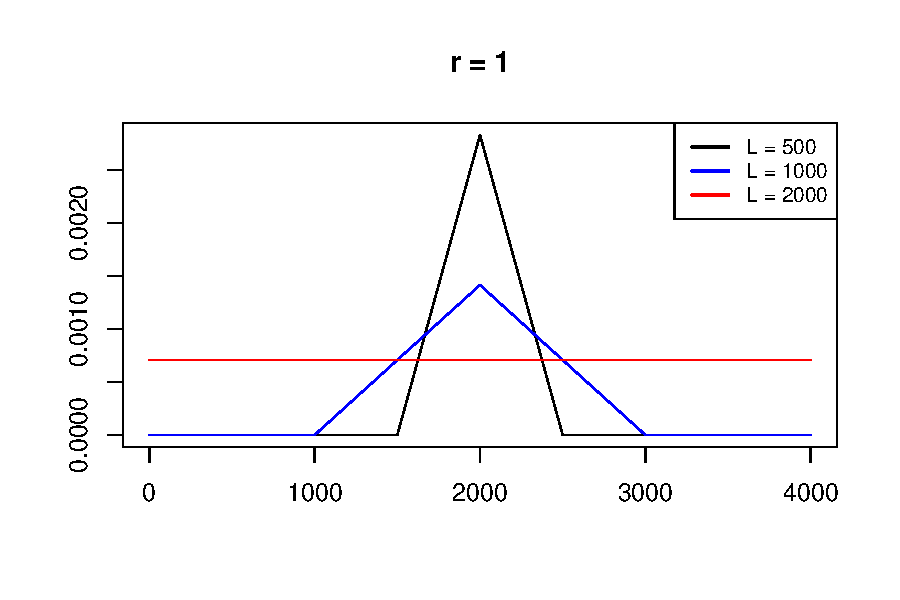
\includegraphics[width=0.48\textwidth]{img/const_outl_err_1}
        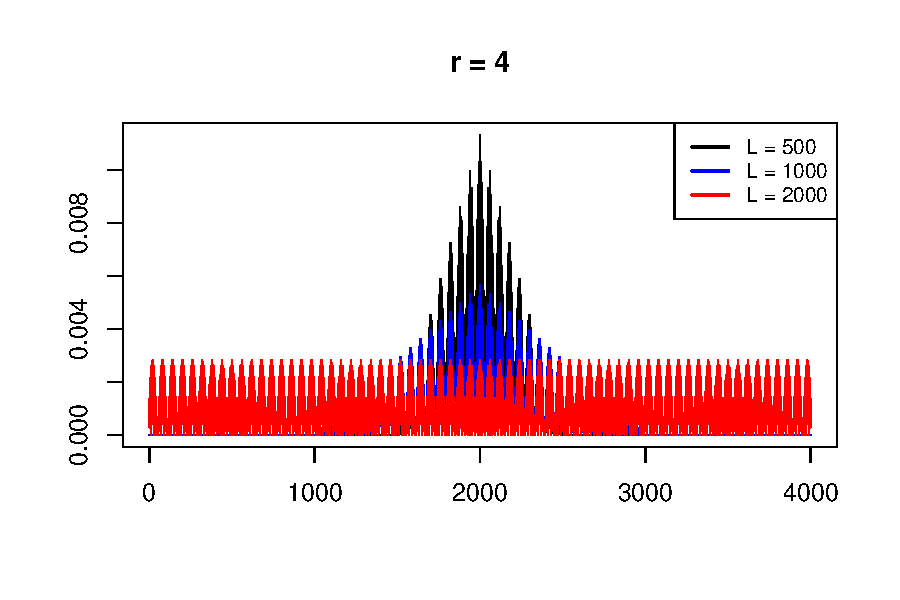
\includegraphics[width=0.48\textwidth]{img/const_outl_err_4}
    \caption{Outlier: Similar squared error behaviour for different ranks $r$.}
    \label{fig:outlier}
\end{figure}

The similar relationship of error variances applies to random noise perturbations. We consider the same signals and the complex Gaussian independent noise with variance 1 for real and imaginary parts. The MSE for $L=1000$ estimated by 500 realisations of the noise is shown in Figure~\ref{fig:noise}. The ratio of the MSE averaging along the series is about 4; this is confirmed by the proximity of the black and blue lines in Figure~\ref{fig:noise}. We also add the line corresponding to the first order error calculated by \eqref{eq:const_noise}. One can see a good agreement between the first-order error and the full error.

\begin{figure}[!htb]
    \centering
        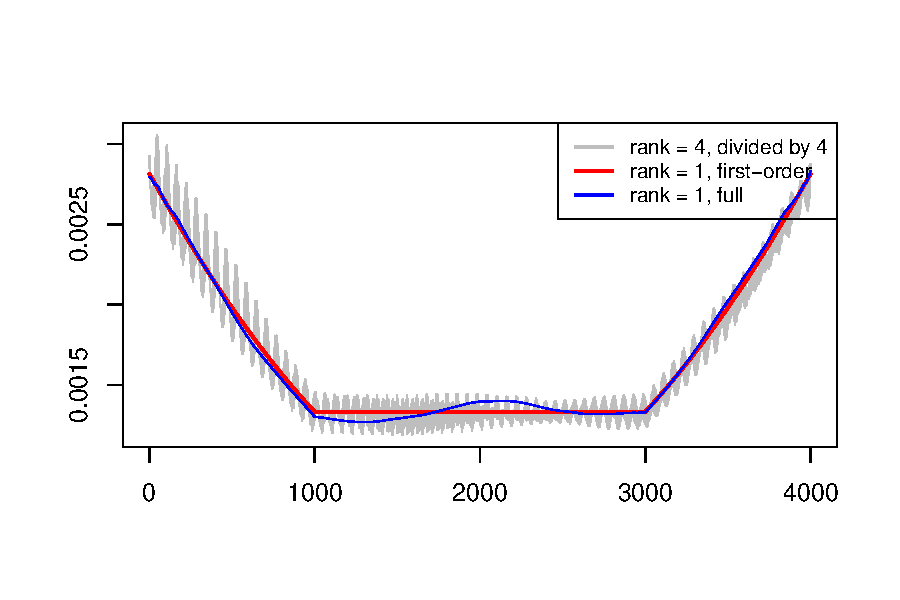
\includegraphics[width=0.6\textwidth]{img/const_noise_err_14}
    \caption{Random noise: Similar error (MSE) behaviour for different ranks $r$.}
    \label{fig:noise}
\end{figure}

All numerical results were obtained using the Rssa package \url{http://CRAN.R-project.org/package=Rssa}. In the implementation of CSSA, the fast numerical method PRIMME was used to compute the truncated SVDs.

\section{Conclusion}
An explicit form of the first-order error of signal estimation at each point was obtained for a constant signal and for both outliers and random noise perturbations. For the random noise, the error was measured by the variance.
It appears that the error does not depend on the signal scale.
For both examples, the proximity between the first-order error and the full error was confirmed numerically.

We have numerically demonstrated how the theoretical results on the accuracy of signal estimation in the simple case of a constant signal help to understand the error behaviour in the general case.
These numerical results allow the use of the proposed error formulas in a general case and appear promising for obtaining theoretical results for rank larger than one.

%\renewcommand\refname{References}

\bibliographystyle{Definitions/mdpi}

	\bibliography{cssa_itise}

\end{document}


